% !TeX root = ../dokumentation.tex

\addchap{\langanhang}
\addsec{1. Teil der Bewertung: Excel-Formular zur schematischen Bewertung einer Arbeit\cite{DHBW-Teil1:2015}}\label{apx:DHBW-Teil1}
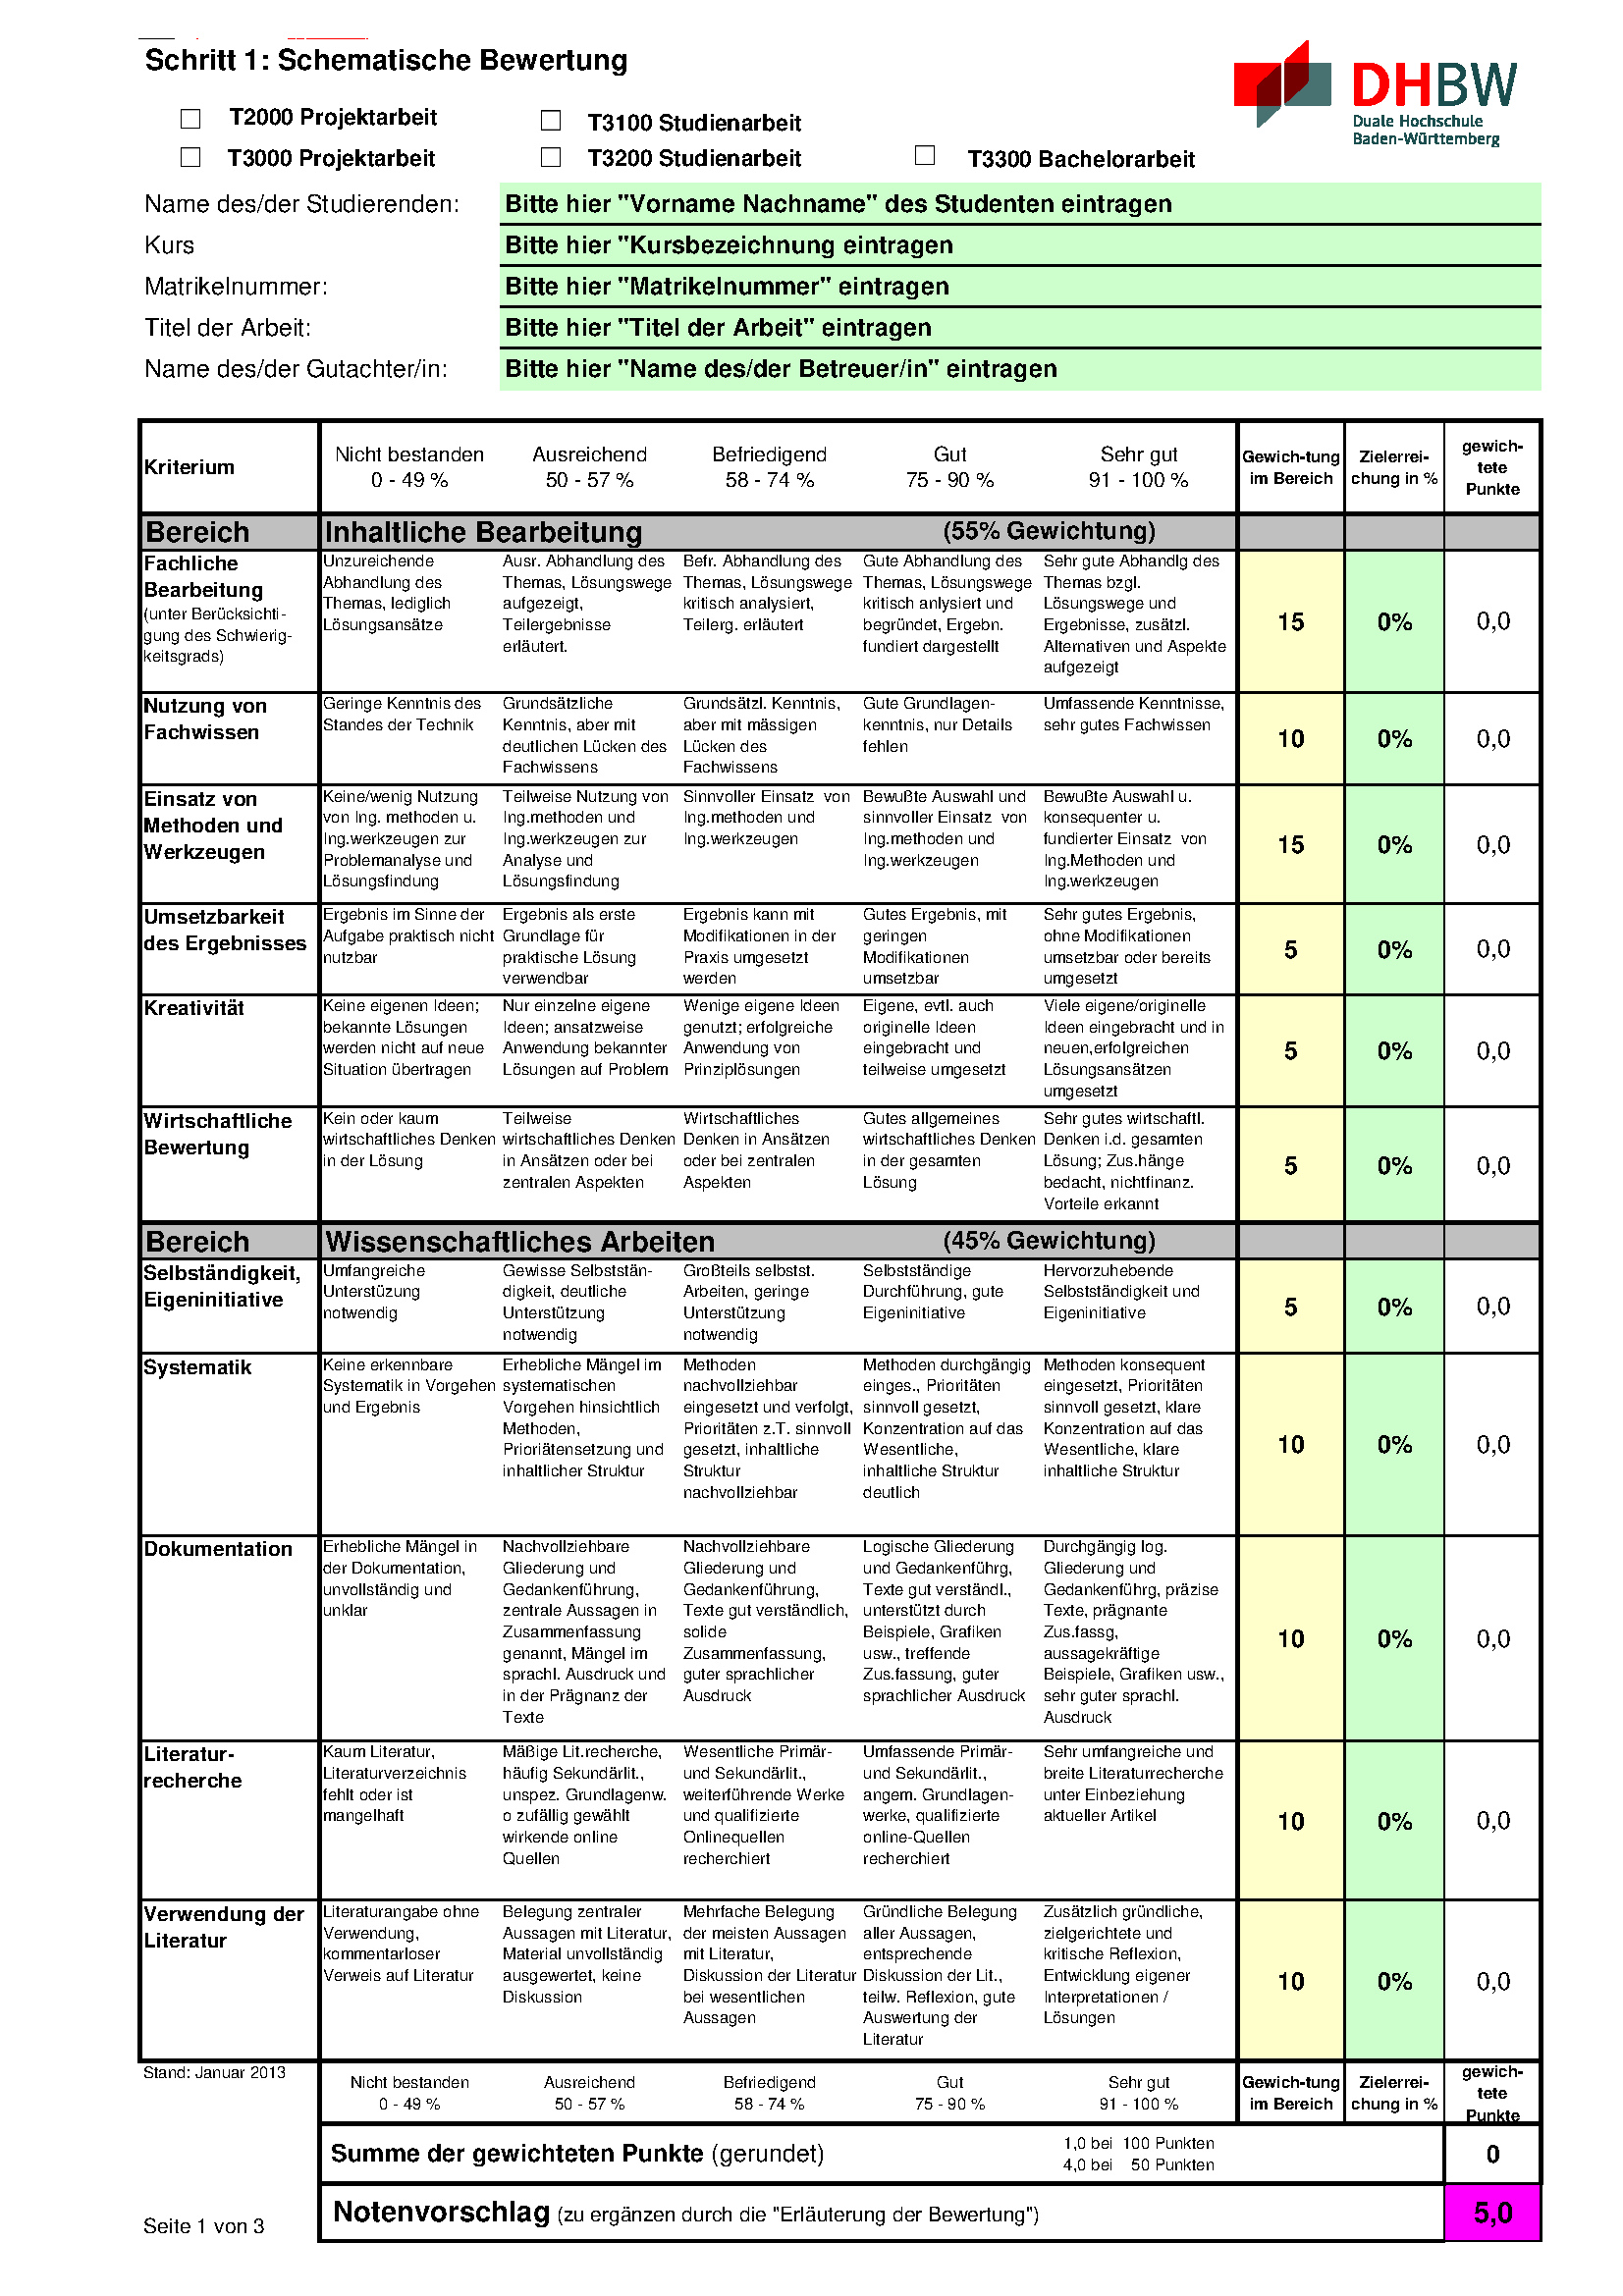
\includepdf[pages=1,scale=.9,pagecommand={}]{images/Bewertung_Projekt_Studien_Bachelor.pdf} % PDF um 10% verkleinert einbinden --> Kopf- und Fußzeile  werden so korrekt dargestellt. Die Option `pages' ermöglicht es, eine bestimmte Sequenz von Seiten (z.B. 2-10 oder `-' für alle Seiten) auszuwählen.
\pagebreak
\addsec{2. Teil der Bewertung: Erläuterung und Kommentare zur Notenfindung \cite{DHBW-Teil2:2015}}\label{apx:DHBW-Teil2}
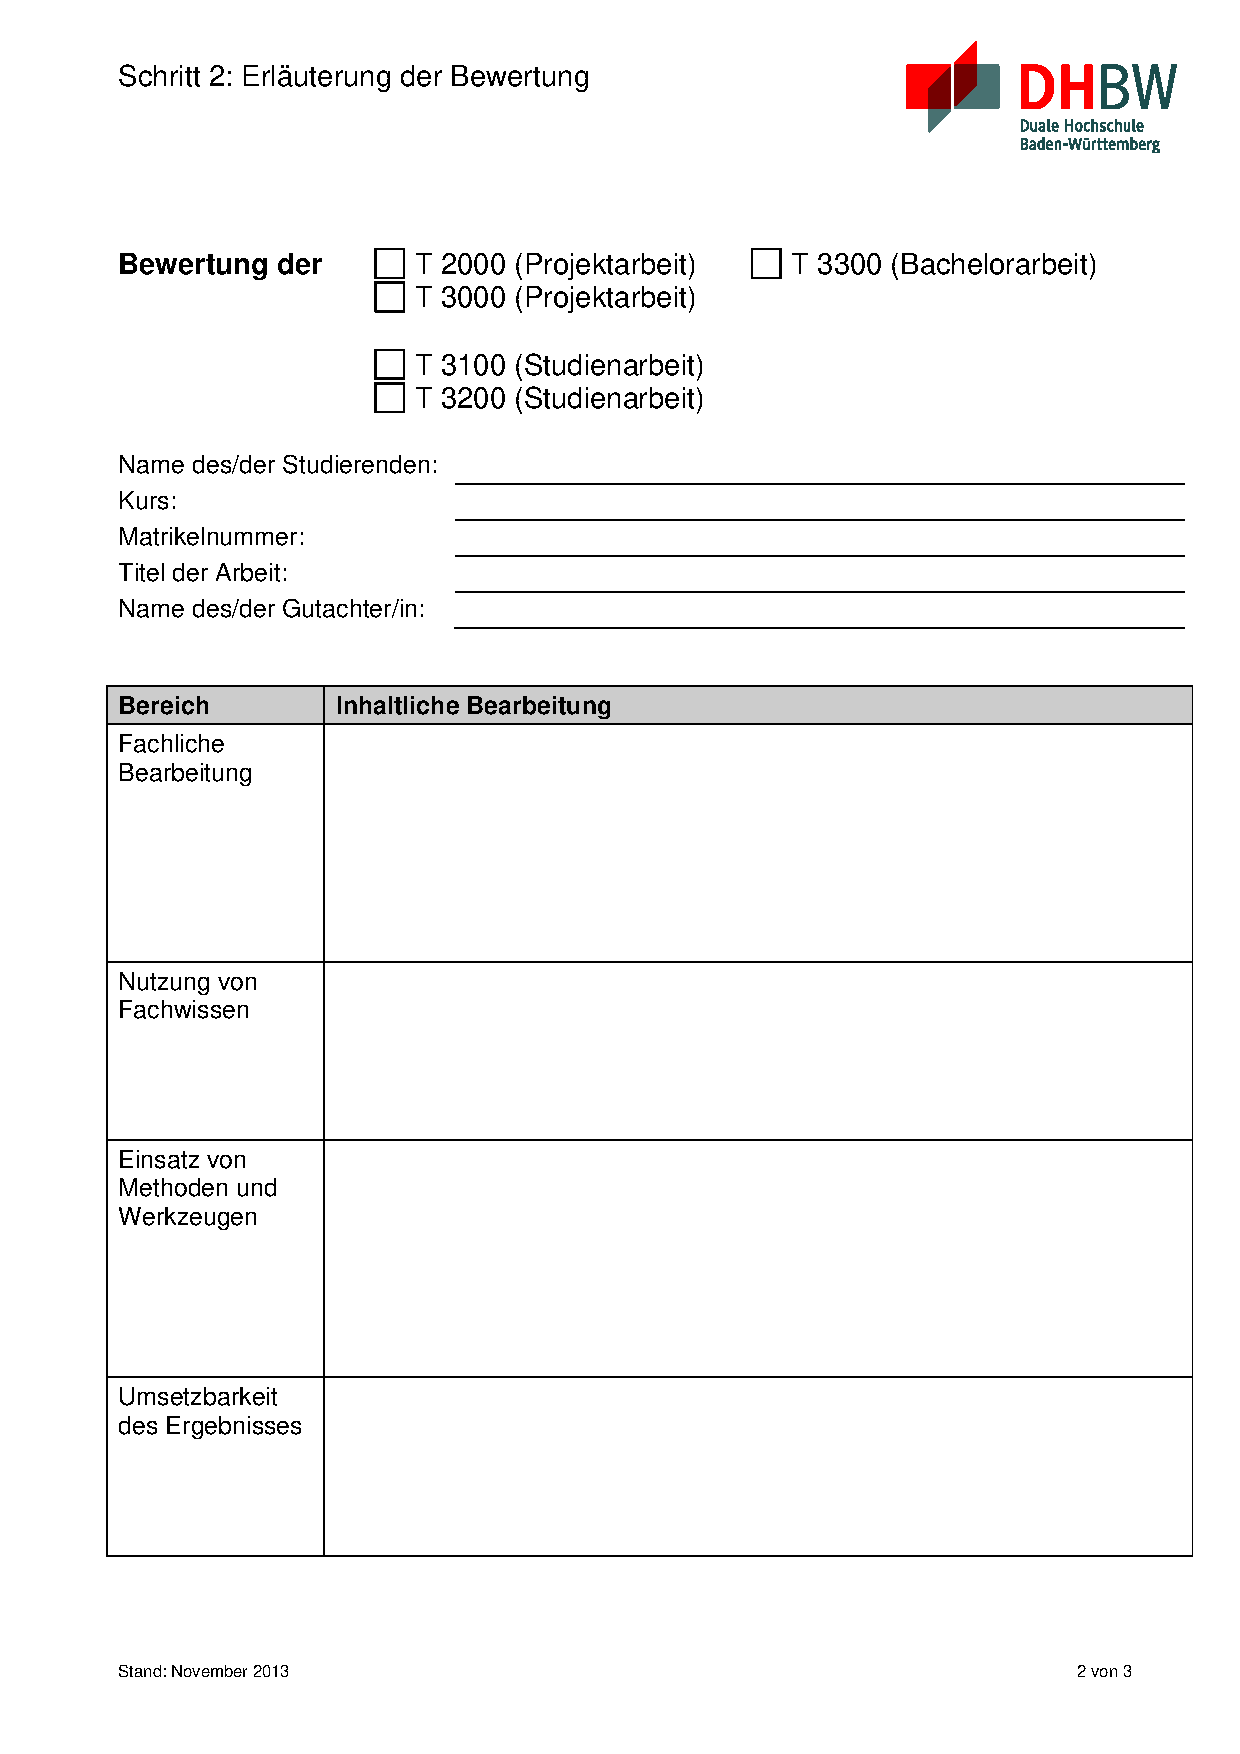
\includepdf[pages=1-2,scale=.9,pagecommand={}]{images/Bewertung_Projekt_Studien_Bachelor_Freitext.pdf} % PDF um 10% verkleinert einbinden --> Kopf- und Fußzeile  werden so korrekt dargestellt. Die Option `pages' ermöglicht es, eine bestimmte Sequenz von Seiten (z.B. 2-10 oder `-' für alle Seiten) auszuwählen.
